%% 
%% Copyright 2007, 2008, 2009 Elsevier Ltd
%% 
%% This file is part of the 'Elsarticle Bundle'.
%% ---------------------------------------------
%% 
%% It may be distributed under the conditions of the LaTeX Project Public
%% License, either version 1.2 of this license or (at your option) any
%% later version.  The latest version of this license is in
%%    http://www.latex-project.org/lppl.txt
%% and version 1.2 or later is part of all distributions of LaTeX
%% version 1999/12/01 or later.
%% 
%% The list of all files belonging to the 'Elsarticle Bundle' is
%% given in the file `manifest.txt'.
%% 

%% Template article for Elsevier's document class `elsarticle'
%% with numbered style bibliographic references
%% SP 2008/03/01

\documentclass[preprint,12pt, a4paper]{elsarticle}

%% Use the option review to obtain double line spacing
%% \documentclass[authoryear,preprint,review,12pt]{elsarticle}

%% For including figures, graphicx.sty has been loaded in
%% elsarticle.cls. If you prefer to use the old commands
%% please give \usepackage{epsfig}

%% The amssymb package provides various useful mathematical symbols
\usepackage{amssymb}
\usepackage{hyperref}
\usepackage{lipsum}
%% The amsthm package provides extended theorem environments
%% \usepackage{amsthm}

%% The lineno packages adds line numbers. Start line numbering with
%% \begin{linenumbers}, end it with \end{linenumbers}. Or switch it on
%% for the whole article with \linenumbers.
%\usepackage{lineno}

%I added these packages
\usepackage{graphicx}
\usepackage{caption}
\usepackage{subcaption}
\usepackage{verbatim}
\usepackage{graphicx}
\usepackage[table,xcdraw]{xcolor}

\journal{Software X}

\begin{document}

\begin{frontmatter}

%% Title, authors and addresses

%% use the tnoteref command within \title for footnotes;
%% use the tnotetext command for theassociated footnote;
%% use the fnref command within \author or \address for footnotes;
%% use the fntext command for theassociated footnote;
%% use the corref command within \author for corresponding author footnotes;
%% use the cortext command for theassociated footnote;
%% use the ead command for the email address,
%% and the form \ead[url] for the home page:
%% \title{Title\tnoteref{label1}}
%% \tnotetext[label1]{}
%% \author{Name\corref{cor1}\fnref{label2}}
%% \ead{email address}
%% \ead[url]{home page}
%% \fntext[label2]{}
%% \cortext[cor1]{}
%% \address{Address\fnref{label3}}
%% \fntext[label3]{}



\title{Spot Report: Real-time Pygame Based Secondary Task For Use In Human-Robot Interaction User Experiments}

%% use optional labels to link authors explicitly to addresses:
%% \author[label1,label2]{}
%% \address[label1]{}
%% \address[label2]{}

\author[a]{Arsha Ali}
\ead{arshaali@umich.edu}
\author[a]{Rohit Banerjee}
\ead{rohitban@umich.edu}
\author[a]{Wonse Jo}
\ead{wonse@umich.edu}
\author[b]{\textcolor{red}{TBD}}
\ead{tbd@tbd.com}
\author[c]{\textcolor{red}{TBD}}
\ead{tbd@tbd.edu}
\author[a]{Lionel P. Robert Jr.}
\ead{lprobert@umich.edu}
\author[a]{Dawn Tilbury}
\ead{tilbury@umich.edu}


\address[a]{Robotics Department, University of Michigan, Ann Arbor, MI, 48109, USA}
\address[b]{\textcolor{red}{Affiliation and address TBD}}
\address[c]{\textcolor{red}{Affiliation and address TBD}}


\begin{abstract}
This paper presents the spot report task as a secondary task for use in human-robot interaction experiments. The spot report task requires counting target objects in static images. The spot report task can be integrated with a primary task, such as one developed in Unreal Engine, using Lab Streaming Layer (LSL). LSL facilitates real-time communication between the primary task and the spot report task. The spot report task is developed in Python, utilizing the Pygame library along with other libraries and packages. The spot report task has the potential to impact research in various human-robot interaction studies. Although the spot report task is motivated by the military domain, the spot report task and software itself are domain-independent and can impact research in various domains.
\end{abstract}

\begin{keyword}

%% keywords here, in the form: keyword \sep keyword
Secondary Task \sep Human-Robot Interaction \sep Pygame \sep Lab Streaming Layer
%% PACS codes here, in the form: \PACS code \sep code

%% MSC codes here, in the form: \MSC code \sep code
%% or \MSC[2008] code \sep code (2000 is the default)

\end{keyword}


\end{frontmatter}

%\linenumbers


\section{Motivation and Significance}
Humans and robots can work together, combining their strengths to handle tasks \cite{ali2022considerations, ali2022heterogeneous}. In human-robot interaction scenarios, humans are increasingly put in a supervisory role of monitoring semi-autonomous robots. Levels of automation can range from no automation to full automation \cite{sheridan1978human, parasuraman2000model}. In semi-autonomous systems, a robot can operate autonomously under certain conditions, but requires human input or assistance outside of these conditions \cite{Zilberstein_2015}. As a result, semi-autonomous systems provide humans the opportunity to engage in a secondary task. A secondary task is a supplemental activity that is completed in conjunction with the primary task. In user experiments, a secondary task is designed to gather additional data or insights about the user's behavior, preferences, or performance during the experiment \cite{mahr2012contre}. The secondary task is typically related to the primary task in some way and provides researchers with a deeper understanding of the user's experience \cite{COLLET20091041}. Performance on the secondary task provides a measure of the spare capacity not required by the primary task \cite{Kerr1973ProcessingDD}. For example, the score on a secondary task may be an indicator of the cognitive demand or workload of the primary task. 

\vspace{2mm}

One domain where secondary tasks are likely to be engaged in is driving, especially with semi-autonomous vehicles (AV). While the AV is driving itself, the human driver can engage in a non-driving secondary task (NDST), such as texting, checking their emails or surfing the web \cite{van2017priming}. When the AV reaches its capability limit, the human must disengage from their secondary task and takeover control of the vehicle until autonomy becomes available again \cite{merat2012highly}. In the context of human-AV studies, several different NDSTs have been used. NDSTs used in human-AV experiments include watching a video \cite{mok2015emergency, ito2016time, nakajima2017effects}, playing a tablet game \cite{mok2017tunneled, epple2018sooner}, playing a mobile phone game \cite{nakajima2017effects, melcher2015take}, entering meaningless digits on a navigator screen \cite{ito2016time}, transcription \cite{van2017priming, wandtner2018non, wandtner2018effects}, calendar entry \cite{van2017priming},  reading \cite{naujoks2014effect}, verbally speaking \cite{nakajima2017effects, wandtner2018non, wandtner2018effects}, searching for the letter `Q' in a field of `O's \cite{azevedo2020context, azevedo2020comparing, azevedo2021internal}, the standardized visual Surrogate Reference Task (SuRT) \cite{radlmayr2014traffic, feldhutter2017duration, gold2013take}, the standardized cognitive n-back Task \cite{radlmayr2014traffic}, and a twenty questions task \cite{merat2012highly} among others. Several secondary tasks are also used in manual vehicle studies, including sorting candy, identifying and taking out coins, and answering map questions \cite{kern2008cars}. \vspace{2mm}


Secondary tasks can be active or passive. Active secondary tasks require physical and/or mental operation, while passive secondary tasks do not \cite{nakajima2017effects}. However, a binary classification may not be appropriate for all kinds of secondary tasks. For example, conversation includes both a passive component (hearing) and an active component (listening and talking) \cite{nakajima2017effects}. Another way to classify secondary tasks could be in terms of stimulus and response modalities. Wandtner et al. used visual vs. auditory stimulus and manual vs. vocal response modalities for a task of reproducing given sentences \cite{wandtner2018effects}. The auditory-vocal version has users listen to sentences and repeat them verbally, the visual-vocal version displays sentences on a tablet and users read them verbally, and the visual-manual version displays sentences on a tablet and users transcribe them using a keyboard \cite{wandtner2018effects}. \vspace{2mm}

In another domain, the military is increasingly looking to evolve robots from tools into full teammates \cite{DoDroadmap}. By incorporating semi-autonomous unmanned ground vehicles into human teams, there is a potential to decrease risks to human soldiers and enhance overall team capabilities \cite{watson2005autonomous}. However, based upon discussions with military personnel and subject matter experts, there is a need to develop a realistic secondary task tailored to military operations for use in experimental studies. Moreover, the secondary task should be suitable and easy to integrate with various primary tasks. Additionally, it is crucial that information and performance data related to the secondary task are easily and continuously accessible in real-time, as they may impact delegation and performance on the primary task. \vspace{2mm}

To tackle these concerns, we developed a Pygame-based secondary task called the spot report task for integration into human-robot interaction user experiments. The spot report task aims to serve as a realistic and engaging self-paced secondary task and is characterized as an active or visual-manual task. In the spot report task, subjects count five categories of target objects in static images. While the spot report task is motivated by military applications, it can easily be used or modified to suit user experiments across domains. The spot report task can also be integrated with a variety of primary tasks. In addition, the spot report task enables real-time communication and information sharing with a primary task by using the Lab Streaming Layer (LSL).

\begin{figure*}[t]
  \centering  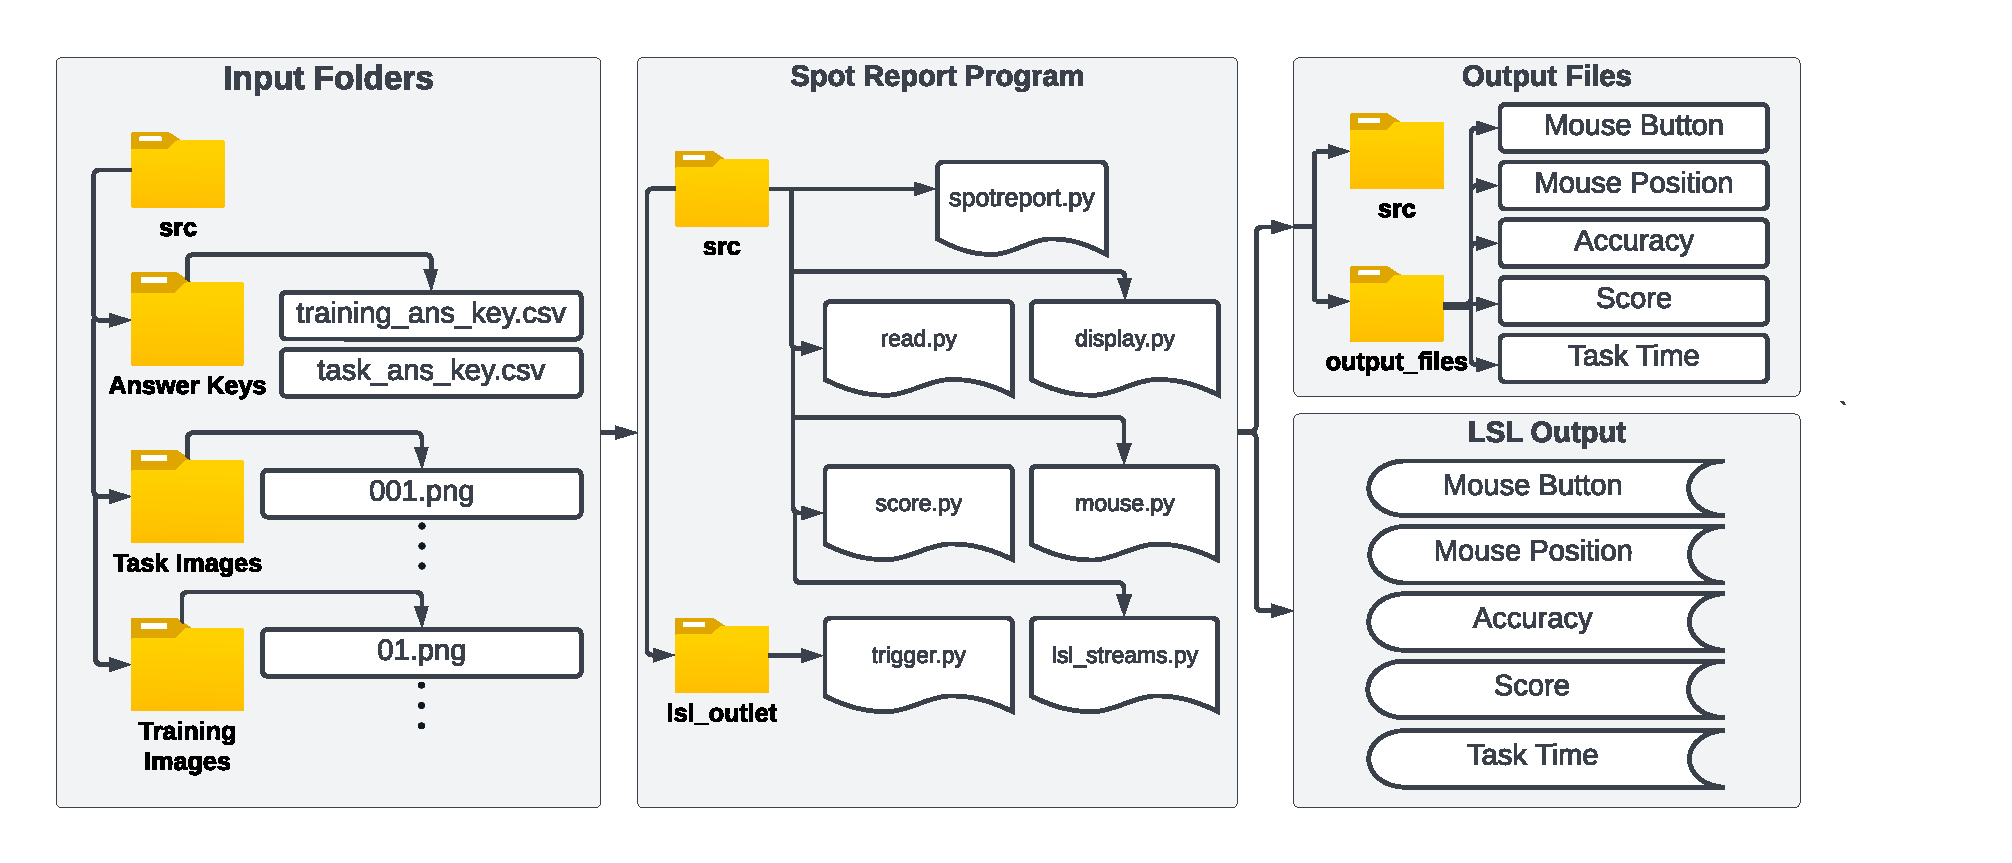
\includegraphics[width=1\linewidth]{Figures/file_structure.pdf}    
  \caption{The file structure of the spot report program. Data is sent to the Lab Streaming Layer (LSL) in real-time when triggered by a corresponding event.}
  \label{fig:file_structure}
\end{figure*}

\section{Software Description}

\subsection{Files}
The file structure of the spot report program is summarized in Fig.\ref{fig:file_structure}. The following files and folders are contained within the \textbf{src} folder. 

\begin{itemize}
    \item \texttt{\textbf{training\_images}}: The training images used in the spot report task are stored in this folder. There are 5 training images, named incrementally from \texttt{01.png} to \texttt{05.png}. The training images are used to train users on the spot report task.

    \item \texttt{\textbf{task\_images}}: The task images used in the spot report task are stored in this folder. There are 165 task images, named incrementally from \texttt{001.png} to \texttt{165.png}. The task images are used during experimentation.
    
    \item \texttt{\textbf{answer\_keys}}: This folder contains the correct count of each object category for each image. The correct counts for the training images are in \textit{\texttt{training\_ans\_key.csv}} and the correct counts for the task images are in \textit{\texttt{task\_ans\_key.csv}}.

    \item \texttt{spotreport.py}: This is the main program running the spot report task. This file references the other files to run the program.

    \item \texttt{read.py}: The images and answer keys are read using this file. For user convenience, an array of optional input arguments can be used to modify the spot report task for a particular domain and move display objects to suit different device screens.

    \item \texttt{display.py}: This file sets up and updates the display for the spot report task. This includes the buttons and labels used throughout the program. Additionally, there is a function to check whether the user has clicked a button.
    
    \item \texttt{score.py}: The score file specifies how each image is scored depending upon the counts entered by the user for each target object category. It also outputs the accuracy, time spent on each task image, and total score.

    \item \texttt{mouse.py}: The mouse file outputs the mouse cursor position and the status of a mouse button as pressed or released.

    \item \texttt{lsl\_streams.py}: This file initializes the LSL inlet and outlet streams. Additionally, this file publishes data from the spot report task on the outlet streams and can receive data from a primary task on the inlet stream.

    \item \texttt{lsl\_outlet}: This folder contains \texttt{trigger.py}, which is an example of how to send data from a primary task to the spot report task using LSL.

    \item \texttt{output\_files}: This folder contains the output csv files that are saved by the spot report task during experimentation.
    
    \item \texttt{randomize\_images.py}: This file is used to randomly rename the 165 task images, which will change the order in which the task images appear in the spot report task. This code is independent of the other files and is therefore not shown in Fig. \ref{fig:file_structure}.

    \item \texttt{resource}: This folder contains \texttt{examples.png}, which is an image that is displayed on the spot report menu that provides examples of the target objects. This file has no effect on the functionality of the spot report task and is therefore not shown in Fig. \ref{fig:file_structure}.
\end{itemize}


\subsection{Software Architecture}
The spot report task is developed in the Python language \cite{vanPython} using the pygame library v2.4.0 {\cite{sweigart2012making}}. The spot report program is summarized by the flowchart in Fig. \ref{fig:flowchart}. The three main screens of the spot report are the menu, training, and task.

\begin{figure}[t]
    \centering
    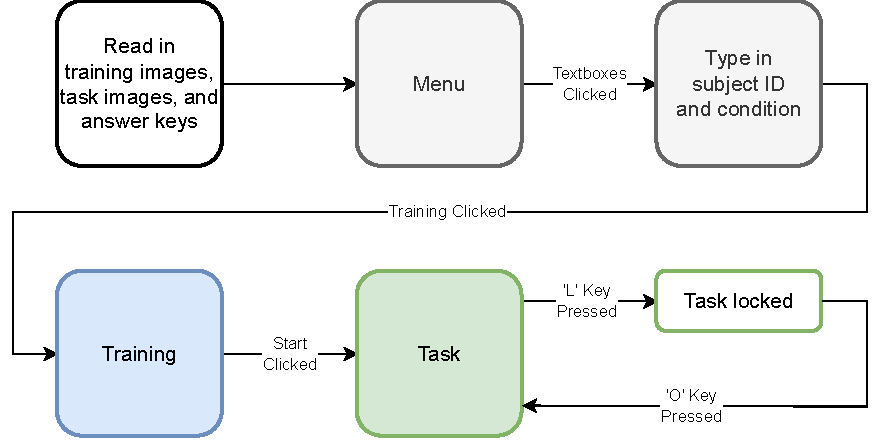
\includegraphics[width=0.95\linewidth]{Figures/software architecture.pdf}
    \caption{A summarized flowchart of the spot report program.}
    \label{fig:flowchart}
\end{figure}

\subsubsection{Menu}
Pygame is initialized upon launching the spot report task, the answer keys are read in as dictionaries, and the training and task images are read in as pygame surface objects stored in lists. The menu is displayed using rectangular and text objects that are drawn onto the screen. Events are monitored through a loop to detect when a mouse button is pressed over the subject ID and condition rectangular objects. The pressing of the left mouse button over the subject ID or condition objects stores the following keyboard input as a string and copies it onto the screen for the corresponding object. Through this method, the subject ID and condition appear as fillable text boxes to the user and rectangular objects appear as clickable buttons. Pressing the escape key or clicking the exit button from the menu will close the entire spot report program.

\subsubsection{Training}
Once the subject ID and condition have been entered, the Training button can be clicked using the left mouse button to enter into the training loop. For training, the screen is set up with a training image to count objects in, plus and minus buttons to increment or decrement the counts of the target object categories, labels and counts for the target object categories, a Next button to advance to the next training image, and a label for the current score. The plus and minus buttons can be used to change the count of a target object category between 0 to 5. When the Next button is clicked, the score is updated and the next training image is shown. After the user has seen all 5 training images, the spot report program returns to the menu. Pressing the escape key or clicking the exit button during training will return the user to the menu.

\subsubsection{Task}
After completing training, the user can click the Start button to begin the experimental spot report task. The spot report task is set up the same as in training, but the task images are used instead of the training images. Additionally, if the user has seen all 165 task images, the task images repeat from the beginning. When the Next button is clicked, the output files for accuracy, score, and task time are updated. Pressing the escape key or clicking the exit button during the task will close the entire spot report program. Pressing the `L' key during the task will lock the spot report task, and pressed the `O' key will unlock the spot report task. When locked, the user is prevented from seeing and interacting with the spot report task. 


\subsection{Images}
The training and task images were developed using Unreal Engine v5.0.3 {\cite{7836249}}. There are five categories of objects that can be present in each image: people, vehicles, bags, barrels, and antennas. In each image, there are between 0 to 5 objects belonging to each category. There are between 0 to 10 total objects in each image. \vspace{2mm}

Across all 165 task images, the number of people, vehicles, bags, barrels, and antennas appear equally as often. In other words, no object category appears more frequently than another. Also, the number of images with a total of $i$ objects is the same as the number of images with a total of $j$ objects, $i,j \in \{0,10\}$. In other words, 15 of the task images have a total of 0 objects, 15 task images have a total of 1 object, and so on, until 15 task images remain with a total of 10 objects.

% Rohit, can you add 6 images at here?

\subsection{Point Scoring}
In the current implementation, the performance of a user on the spot report task is determined through a point scoring system. In order to earn points, the user must first submit the correct count for a target object category based on the objects in the image. Then, the user earns 1 point times the number of objects present for the categories of vehicles, bags, barrels, and antennas. People are considered to be more important target objects, so for correctly counting the number of people in an image, the user earns 2 points times the number of people in the image. If the user correctly counts all target object categories for an image, 1 bonus point is awarded. The point scoring system is summarized in Table \ref{tab:points}. Although this is the way we have designed the point scoring system, it can easily be adapted for other desired variations in point scoring.

\begin{table}[h]
\caption{Points Earned Through Each Spot Report}
\label{tab:points}

\centering
\begin{tabular}{|l|c|c|c|c|}
    \hline
        \rowcolor[HTML]{C0C0C0} 
    \multicolumn{1}{|c|}{\textbf{Object}}  & \multicolumn{3}{c|}{\textbf{Points}} & \textbf{Bonus}\\
    \hline     \hline

    People & +2  & & &\\
    Vehicles & +1 & & &\\
    Bags & +1 & x number of object & x correct count (0 or 1) & +1\\
    Barrels & +1 & & &\\
    Antennas & +1 & & &\\
    \hline
\end{tabular}
\end{table}



\subsection{Support for Lab Streaming Layer}
Lab Streaming Layer is an open-source software framework that allows researchers to synchronize and stream data between different devices and software applications. It was developed to address the challenges of integrating multiple data streams in research settings, where data is often collected from different sources simultaneously. LSL provides a standardized way of time-stamping and labeling data, making it easier for researchers to combine and analyze data from different sources. It also allows for real-time processing and visualization of data, which can be particularly useful for studies involving human subjects \cite{kothe2014lab}. The LSL inlet and outlet streams are summarized in Table \ref{tab:detail_lsl_streams}.

\begin{table*}[]
\centering
\caption{Details of Lab streaming layer streams used in the sport report program.}
\label{tab:detail_lsl_streams}
\resizebox{\textwidth}{!}{%
\begin{tabular}{|c|c|c|c|c|c|l|}
\hline
\rowcolor[HTML]{EFEFEF} 
\textbf{LSL info.} & \textbf{\begin{tabular}[c]{@{}c@{}}Stream \\ name\end{tabular}} & \textbf{\begin{tabular}[c]{@{}c@{}}Stream \\ type\end{tabular}} & \textbf{\begin{tabular}[c]{@{}c@{}}Channel \\ count\end{tabular}} & \textbf{\begin{tabular}[c]{@{}c@{}}Sampling \\ rate\end{tabular}} & \textbf{Format} & \multicolumn{1}{c|}{\textbf{Details}} \\ \hline
\textbf{Outlet 1} & spt\_mouse\_pos & mouse\_pose & 3 & Irregular & int32 & \begin{tabular}[c]{@{}l@{}}Ch 1: Image ID \\ Ch 2: X position \\ Ch 3: Y position\end{tabular} \\ \hline
\textbf{Outlet 2} & spt\_mouse\_btn & mouse\_button & 2 & Irregular & int32 & \begin{tabular}[c]{@{}l@{}}Ch 1: Image ID \\ Ch 2: 0 (for released) or 1 (for pressed) \end{tabular} \\ \hline
\textbf{Outlet 3} & spt\_task\_time & task\_time & 2 & Irregular & float32 & \begin{tabular}[c]{@{}l@{}}Ch 1: Image ID\\ Ch 2: Execution time (sec)\end{tabular} \\ \hline
\textbf{Outlet 4} & spt\_task\_accuracy & task\_accuracy & 9 & Irregular & float32 & \begin{tabular}[c]{@{}l@{}}Ch 1: Image ID \\ Ch 2: Correct counts\\ Ch 3: Incorrect counts\\ Ch 4: Accuracy {[}\%{]}\\ Ch 5: count of people \\ Ch 6: count of vehicles \\ Ch 7: count of bags \\ Ch 8: count of barrels \\ Ch 9: count of antennas \end{tabular} \\ \hline 
\textbf{Outlet 5} & spt\_total\_score & total\_score & 3 & Irregular & int32 & \begin{tabular}[c]{@{}l@{}}Ch 1: Image ID \\ Ch 2: Image score\\ Ch 3: Total score \end{tabular} \\ \hline \hline
\rowcolor[HTML]{EFEFEF} 
\textbf{Inlet 1} & spt\_task\_trigger & start\_pause\_task & 1 & Irregular & int32 & \begin{tabular}[c]{@{}l@{}}0 (to unlock task)\\ 1 (to lock task)\end{tabular} \\ \hline
\end{tabular}%
}
\end{table*}

\subsubsection{Inlet LSL stream}
\vspace{2mm}
The spot report program is controlled by an inlet stream called \texttt{spt\_task\_\\trigger}. This stream allows the user to lock or unlock the spot report task. Two variables, 0 and 1, are associated with specific roles:

\begin{itemize}
    \item 0: Unlocks the spot report task. When a data sample with the value 0 is received through the \texttt{spt\_task\_trigger} inlet stream, the spot report task will unlock to the user.
    \item 1: Locks the spot report task. When a data sample with the value 1 is received through the \texttt{spt\_task\_trigger} inlet stream, the spot report task will lock to the user.
\end{itemize}

By sending the appropriate value (0 or 1) through the \texttt{spt\_task\_trigger} inlet stream, the user can control the spot report task and manage its execution state. This functionality represents how a primary task can influence the spot report task, and is provided in addition to using the `L' key to lock and the `O' key to unlock the spot report task.


    
\subsubsection{Outlet LSL streams}
\vspace{2mm}

\textit{Mouse information:} The spot report task sends cursor positions (X and Y coordinates within the window) and mouse button clicks at irregular intervals once the experimental spot report task is initiated after training. Mouse information is transmitted through the \texttt{spt\_mouse\_pos} outlet stream for cursor positions and through the \texttt{spt\_mouse\_btn} outlet stream for mouse button clicks.

\vspace{2mm}

\textit{Task performance:} We provide 165 task images to be displayed during the spot report task, along with the corresponding answers saved in the \texttt{answer\_keys} directory. Upon clicking the Next button, the execution time in seconds, accuracy, and score information is sent on the outlet streams. Execution time, accuracy, and score information are transmitted through the \texttt{spt\_task\_time}, \texttt{spt\_task\_accuracy}, and \texttt{spt\_total\_score} outlet streams respectively.  


\subsection{Output Files and Data}
The output files \texttt{task\_time.csv}, \texttt{accuracy.csv}, and \texttt{score.csv} log the execution time, accuracy, and score information, along with the current date and time and the image ID. These values are logged every time the Next button is clicked. The score can also be logged by a change in points caused by a primary task, for example, if such information is sent on an LSL inlet stream. The output files \texttt{mouse\_pos.csv} and \texttt{mouse\_button.csv} logs the mouse cursor position and the state of the mouse button, along with the current date and time and the image ID. These values are logged every time the mouse cursor position changes or a mouse button is pressed or released. Each of these output file names are appended with the subject ID and condition typed into the menu textboxes as \texttt{\_S$<$subject ID$>$\_C$<$condition$>$} to automatically save data from different users. All output files are stored in the \texttt{output\_files} folder. Note that these output files log mouse information and task performance data from the task images after clicking the Start button. No information from the menu or training is recorded.

\begin{figure}[t]
    \centering
    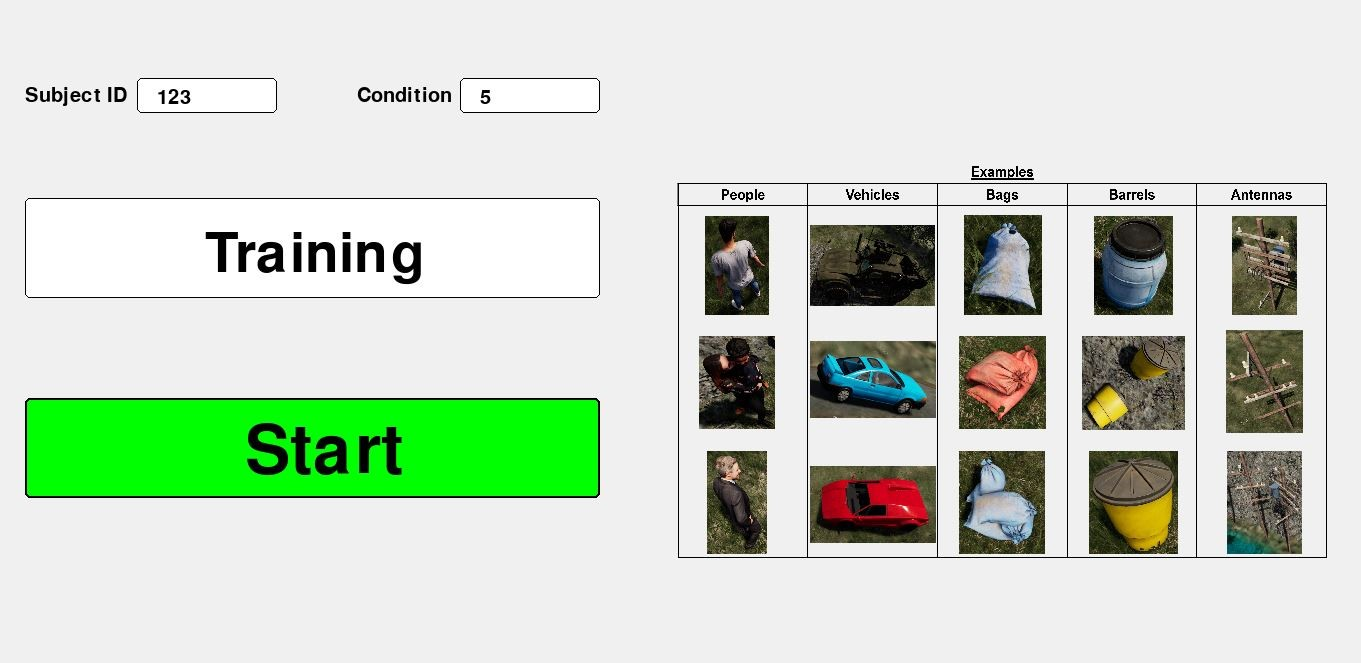
\includegraphics[width=1.0\textwidth]{Figures/menu.jpg}
    \caption{The spot report menu. The user types in the subject ID (example: 123) and condition (example: 5). Then, the user can click the Training button to begin training. Then, the user can click the Start button to begin the spot report task.}
    \label{fig:menu}
\end{figure}

\section{Illustrative Examples}
We conducted testing of the spot report program using Python v3.9.7 in Visual Studio Code. A video of the spot report program is available at \url{https://youtu.be/mhUKsqkuMPQ}. The program can be executed from the terminal by entering \texttt{python .\textbackslash spotreport.py} from the \texttt{src} folder and optionally providing the command line arguments defined in the \texttt{read.py} file. This will launch the spot report program and present the menu, as depicted in Fig. \ref{fig:menu}. To enable the Training button, a subject ID and condition must be entered into the text boxes on the menu. After completing the training, the program will return to the menu. Training needs to be completed at least once before the Start button can be clicked to initiate the spot report task with the task images. \vspace{0.1mm}

\begin{figure*}[!h]
        \centering
        \begin{subfigure}{0.71\linewidth}
            \centering
            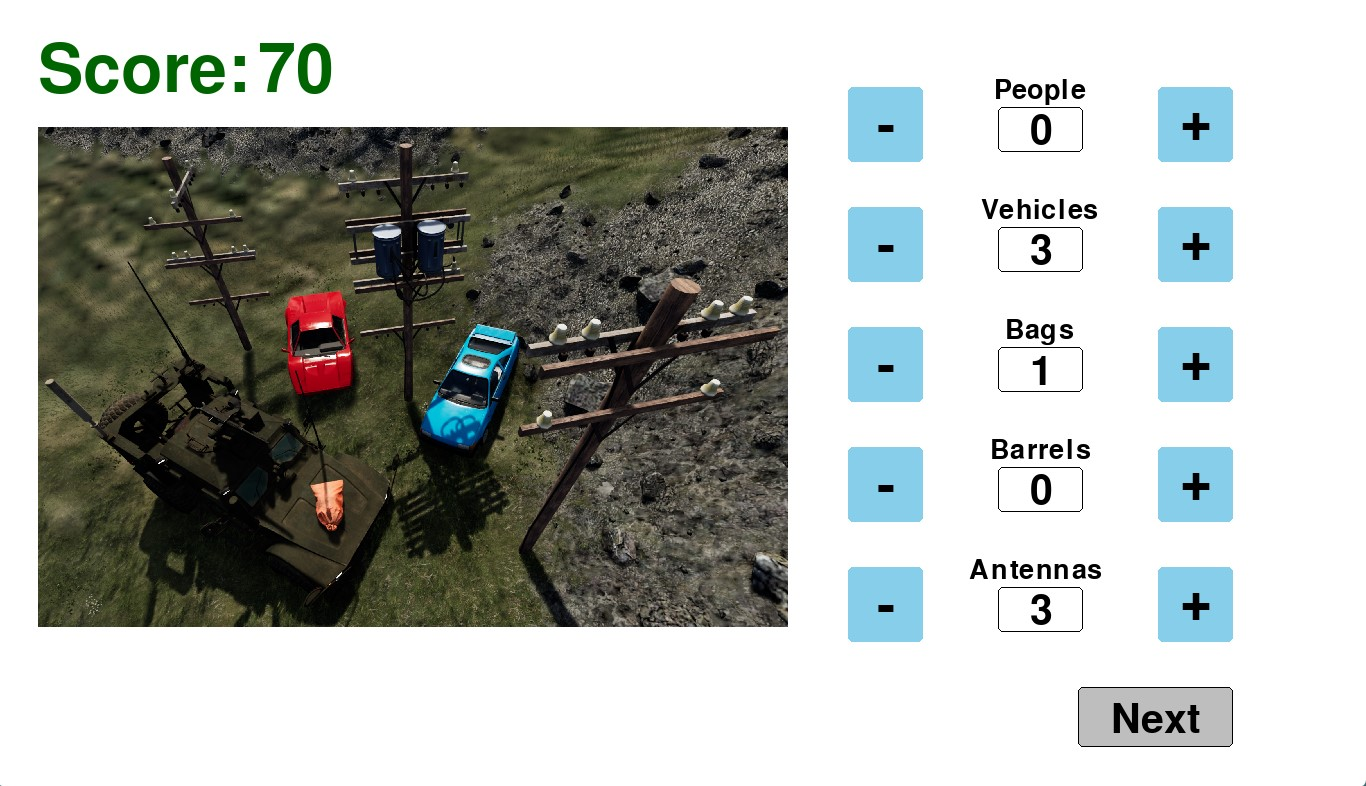
\includegraphics[width=0.96\linewidth]{Figures/exA.jpg}
            \caption{An example where the user has counted all objects correctly.}
            \label{fig:examplesA}
        \end{subfigure}
        \begin{subfigure}{0.71\linewidth}
            \centering
            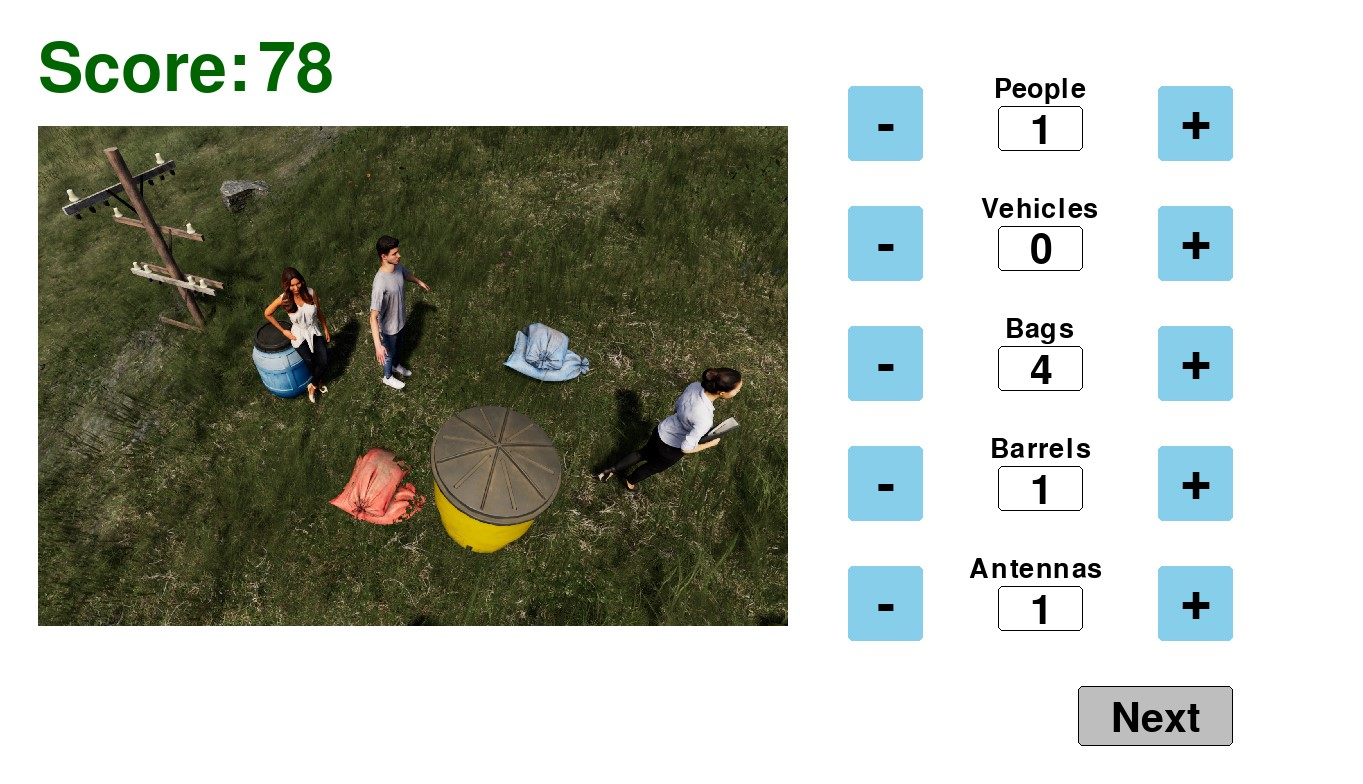
\includegraphics[width=0.96\linewidth]{Figures/exB.jpg}
            \caption{An example where the user has correctly counted the number of vehicles, bags, and antennas but incorrectly counted the number of people and barrels.}
            \label{fig:examplesB}
        \end{subfigure}
        \begin{subfigure}{0.71\linewidth}
            \centering
            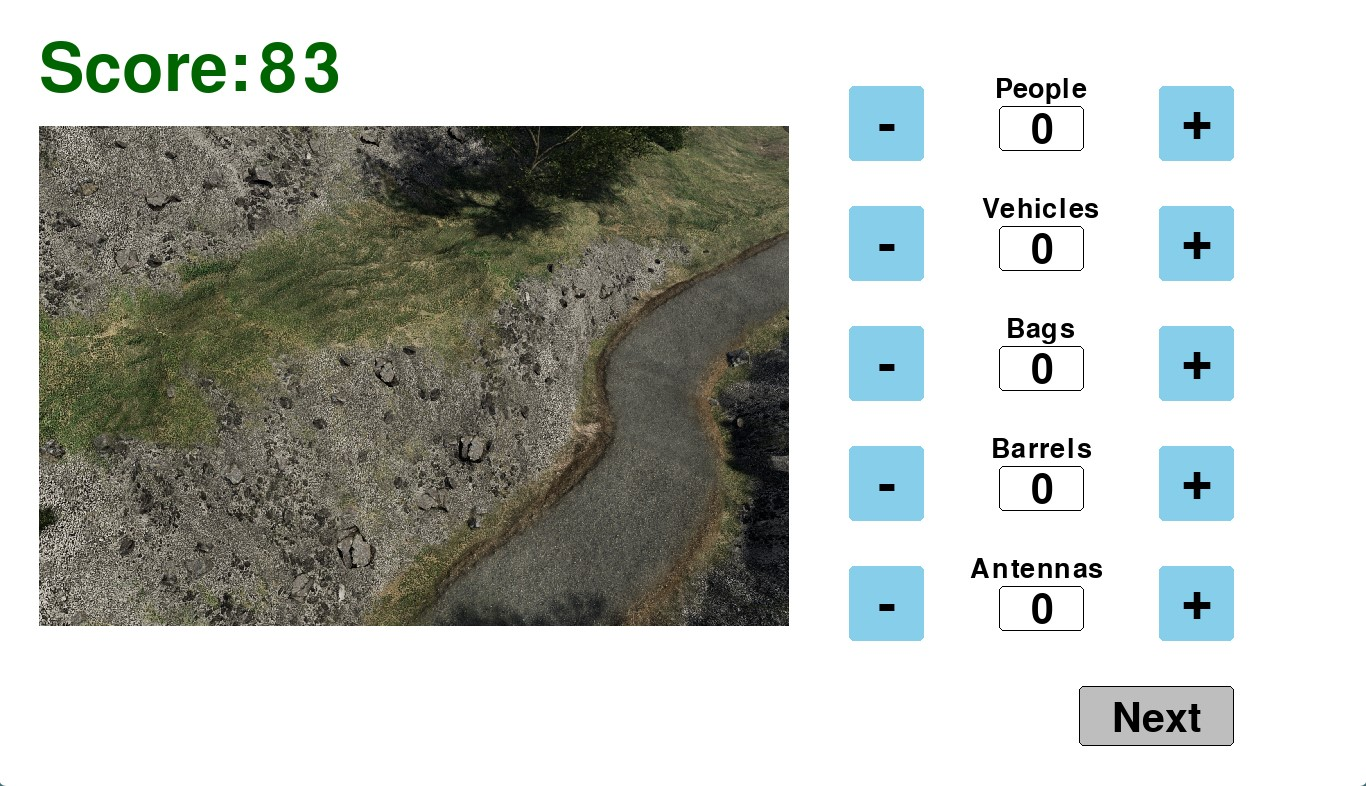
\includegraphics[width=0.96\linewidth]{Figures/exC.jpg}
            \caption{An example where there are no objects in the image and the user has correctly left all object categories with a count of 0.}
            \label{fig:examplesC}
        \end{subfigure}
        \caption{\label{fig:examples} Three examples of the spot report task with object counts filled in by the user.}
\end{figure*}
   

Three examples of the spot report task are shown in Fig. \ref{fig:examples}, and example counts that could be submitted by a user are listed in Table \ref{tab:example_counts}. The correct counts for each of the three examples is listed in Table \ref{tab:example_answers}. The calculation of the number of points earned in each of these three examples is shown in Table \ref{tab:example_points}. In example A in Fig. \ref{fig:examplesA}, all of the object categories are counted correctly and the 1 point bonus is earned. In example B Fig. \ref{fig:examplesB}, the number of people and barrels are incorrectly counted so no points are earned from the people or barrel categories and the bonus is not earned. Points are still earned from correctly counting the other object categories. In example C in Fig. \ref{fig:examplesC}, there are no objects in the image and all of the object categories are counted correctly as 0 so the bonus of 1 point is earned.


\begin{comment}
\begin{figure}[t]
    \centering
    \begin{subfigure}{0.32\linewidth}
        \centering
        \includegraphics[width=1\linewidth]{Figures/sport_report_task/001.png}
        \label{fig:exA}
    \end{subfigure}
    \begin{subfigure}{0.32\linewidth}
        \centering
        \includegraphics[width=1\linewidth]{Figures/sport_report_task/002.png}
        \label{fig:exB}
    \end{subfigure}
    \begin{subfigure}{0.32\linewidth}
        \centering
        \includegraphics[width=1\linewidth]{Figures/sport_report_task/003.png}
        \label{fig:exB}
    \end{subfigure}
    
    \begin{subfigure}{0.32\linewidth}
        \centering
        \includegraphics[width=1\linewidth]{Figures/sport_report_task/004.png}
        \label{fig:exC}
    \end{subfigure}
    \begin{subfigure}{0.32\linewidth}
        \centering
        \includegraphics[width=1\linewidth]{Figures/sport_report_task/005.png}
        \label{fig:exC}
    \end{subfigure}
    \begin{subfigure}{0.32\linewidth}
        \centering
        \includegraphics[width=1\linewidth]{Figures/sport_report_task/006.png}
        \label{fig:exB}
    \end{subfigure}
    \caption{Examples of images used in the spot report task \cite{}.}
    \label{fig:exB}
\end{figure}
\end{comment}


\begin{table}[h]
\caption{Example Counts Submitted by User for Example Task Images}
\label{tab:example_counts}
\centering
\begin{tabular}{|c|c|c|c|c|c|}
    \hline

    \rowcolor[HTML]{C0C0C0} 

    \textbf{Example} & \textbf{People} & \textbf{Vehicles} & \textbf{Bags} & \textbf{Barrels} & \textbf{Antennas} \\
    \hline     \hline

    A & 0 & 3 & 1 & 0 & 3 \\
    \hline
    B & 1 & 0 & 4 & 1 & 1 \\
    \hline
    C & 0 & 0 & 0 & 0 & 0 \\
    \hline
\end{tabular}
\end{table}


\begin{table}[h]
\caption{Correct Counts for Example Task Images}
\label{tab:example_answers}
\centering
\begin{tabular}{|c|c|c|c|c|c|}
    \hline
    \rowcolor[HTML]{C0C0C0} 

    \textbf{Example} & \textbf{People} & \textbf{Vehicles} & \textbf{Bags} & \textbf{Barrels} & \textbf{Antennas} \\
    \hline    \hline

    A & 0 & 3 & 1 & 0 & 3 \\
    \hline
    B & 3 & 0 & 4 & 2 & 1 \\
    \hline
    C & 0 & 0 & 0 & 0 & 0 \\
    \hline
\end{tabular}
\end{table}


\begin{table}[h]
\caption{Points Earned in Example Task Images}
\label{tab:example_points}
\centering
\resizebox{0.95\textwidth}{!}{%
\begin{tabular}{|c|p{1.6cm}|c|c|c|c|c|}
    \hline
    \rowcolor[HTML]{C0C0C0} 

    \textbf{Example} & \textbf{Object} & \textbf{Points} & \textbf{\begin{tabular}[c]{@{}c@{}}Number \\ of Object\end{tabular}} & \textbf{\begin{tabular}[c]{@{}c@{}}Correct \\Count\end{tabular}} & \textbf{Bonus} & \textbf{\begin{tabular}[c]{@{}c@{}}Points \\Earned\end{tabular} } \\
    \hline    \hline

    & People & 2 &      0 & 1 & & \\
    & Vehicles & 1 &    3 & 1 & & \\
    A & Bags & 1 &      1 & 1 & 1 & 8 \\
    & Barrels & 1 &     0 & 1 & & \\
    & Antennas & 1 &    3 & 1 & & \\
    \hline
    \hline
    \rowcolor[HTML]{EFEFEF} & People & 2 &      3 & 0 & & \\
    \rowcolor[HTML]{EFEFEF} & Vehicles & 1 &    0 & 1 & & \\
    \rowcolor[HTML]{EFEFEF} B & Bags & 1 &      4 & 1 & 0 & 5 \\
    \rowcolor[HTML]{EFEFEF} & Barrels & 1 &     2 & 0 & & \\
    \rowcolor[HTML]{EFEFEF} & Antennas & 1 &    1 & 1 & & \\
    \hline
    \hline
    & People & 2 &      0 & 1 & & \\
    & Vehicles & 1 &    0 & 1 & & \\
    C & Bags & 1 &      0 & 1 & 1 & 1 \\
    & Barrels & 1 &     0 & 1 & & \\
    & Antennas & 1 &    0 & 1 & & \\
    \hline
\end{tabular}
}
\end{table}


\begin{figure}[h!]
    \centering
    
\includegraphics[scale=0.5]{Figures/locked.jpg}
    \caption{The display when the spot report task is locked.}
    \label{fig:locked}
\end{figure}


The spot report task with the task images can be locked to the user. This can be used to force users to disengage from the secondary task and engage with the primary task. When locked, a black screen with text is displayed as shown in Fig. \ref{fig:locked}.


\section{Impact}
There is a wide range of secondary tasks being used in human-robot interaction user experiments. However, military personnel and subject matter experts have expressed the need for a secondary task that is relevant, engaging, and realistic in military settings. Furthermore, the secondary task should be adaptable to various primary tasks while continuously outputting data, which can be used in real-time by the primary task. The proposed spot report task addresses these requirements. \vspace{2mm}

By providing continuous and readily accessible data, the spot report task has the potential to enhance existing human-robot interaction user experiments and enable new ones. With the spot report task, many research questions and topics in various domains can be pursued and impacted. For instance, the authors are using the spot report task in an ongoing research experiment to study team situational awareness and trust. In this experiment, a human subject collaborates with two semi-autonomous vehicles to carry out the primary task of navigating and searching an off-road environment. When the human subject is not operating either of the semi-autonomous vehicles, they are expected to engage in the spot report task. The human subject is locked out of the spot report task while operating either semi-autonomous vehicle. Both the primary and secondary tasks contribute to the points earned by the human subject.


\section{Conclusions}
In this paper, we present the spot report task as a secondary task for use in human-robot interaction user experiments across domains. The spot report task is self-paced and entails counting target objects in static images. The spot report task also outputs various data in real-time using LSL, which can be seamlessly integrated with a range of primary tasks.

\section*{Declaration of Competing Interest}
The authors declare that they have no known competing financial interests or personal relationships that could have appeared to influence the work reported in this paper.

\section*{Software and Data Availability}
All software files and example outputs, along with paper source code and paper figures, are available in a public repository at \url{https://github.com/UMich-MAVRIC/SpotReport}. 
%No data was used for the research described in this paper.


\section*{Funding}
The authors wish to acknowledge the technical and financial support of the Automotive Research Center (ARC) in accordance with Cooperative Agreement W56HZV-19-2-0001 U.S. Army DEVCOM Ground Vehicle Systems Center (GVSC) Warren, MI.

\section*{Acknowledgements}
We would like to thank \textcolor{red}{TBDa, PhD, TBDb, PhD, and TBDc, PhD} in helping to guide the design of the spot report task and the design of the ongoing user experiment.
%Kayla Riegner, PhD, Jonathon Smereka, PhD, Dariusz Mikulski, PhD, and Samantha Dubrow, PhD
 
%% The Appendices part is started with the command \appendix;
%% appendix sections are then done as normal sections
%% \appendix

%% \section{}
%% \label{}

%% References:
%% If you have bibdatabase file and want bibtex to generate the
%% bibitems, please use
%%
%%  \bibliographystyle{elsarticle-num} 
%%  \bibliography{<your bibdatabase>}

%% else use the following coding to input the bibitems directly in the
%% TeX file.

\bibliographystyle{IEEEtran}
\bibliography{IEEEabrv,ref}


\section*{Current code version}
\label{}

\begin{table}[!h]
\caption{Code metadata}
\label{tab:code_metadata} 
\begin{tabular}{|l|p{6.5cm}|p{6.5cm}|}
\hline
C1 & Current code version & v1.0 \\
\hline
C2 & Permanent link to code/repository used for this code version & \url{https://github.com/UMich-MAVRIC/SpotReport}\\
\hline
C3  & Permanent link to Reproducible Capsule & \url{https://github.com/UMich-MAVRIC/SpotReport}\\
\hline
C4 & Legal Code License   & MIT No Attribution (MIT-0) License \\
\hline
C5 & Code versioning system used & GitHub (git) \\
\hline
C6 & Software code languages, tools, and services used & Python v3.9.7 \\
\hline
C7 & Compilation requirements, operating environments \& dependencies & pygame v2.4.0, pylsl v1.16.1, pandas v2.0.2, numpy v1.24.3, glob, csv, datetime, random, os, time \\
\hline
C8 & If available Link to developer documentation/manual &  \url{https://github.com/UMich-MAVRIC/SpotReport} \\
\hline
C9 & Support email for questions & arshaali@umich.edu\\
\hline
\end{tabular}
\end{table}


\end{document}
\endinput
%%
%% End of file `SoftwareX_article_template.tex'.
